
\section{Neto et al. 2016}
\label{sec:exp-setup}
In \cite{Netoetal}, 2016 they described in detail a procedure for precisely aligning two probes for in vivo “paired-recordings” such that the spiking activity of a single neuron is monitored with both a dense extracellular silicon polytrode and a juxtacellular micro-pipette. A “ground truth” dataset was acquired from rat cortex with 32 and 128-channel silicon polytrodes and it is available online (http://www.kampff-lab.org/validating-electrodes). A brief description of the dual-recording setup design and protocol are presented below. In Section \ref{subsec:Netodataset}, the dataset is presented

\subsection{Set-up design and protocol}
\label{subsec:setup-and-protocol}
In Fig. \ref{fig:experimental-aparatus}a is presented a schematic of the dual-probe recording station where two aligned, multi-axis micromanipulators (Scientifica, UK) and a long working distance optical microscope are required to reliably target neural cell bodies located within $\sim 100 \mu m$ of the polytrode electrode sites without optical guidance. A “PatchStar” (PS) and an “In-Vivo Manipulator” (IVM) are mounted on opposite sides of a rodent stereotaxic frame with different approach angles, $61^{\circ}$  and $-48.61^{\circ}$  from the horizontal, respectively (Fig \ref{fig:experimental-aparatus}b). 

\begin{figure}[htb]
	\centering
	\includegraphics[width=\textwidth]{2.Chapter/experimental-setup-dev.pdf}
	\caption{In vivo paired-recording setup: design and method.
(a) Schematic of the dual-probe recording station. The PS micromanipulator drives the juxtacellular pipette and the IVM manipulator drives the extracellular polytrode. The setup includes a long working distance microscope assembled from optomechanical components mounted on a three-axis motorized stage. The alignment image provides a high-resolution view from above the stereotactic frame, upper left, however a side-view can also be obtained for calibration purposes, upper right (scale bar $100 \mu m$).  (b) Schematic of a coronal view of the craniotomy and durotomies with both probes positioned at the calibration point. The distance between durotomies, such that the probe tips meet at deep layers in cortex, was around 2 mm. The black arrows represent the motion path for both electrodes entering the brain (scale bar 1 mm). (c) Diagram of simultaneous extracellular and juxtacellular paired-recording of the same neuron at a distance of $90 \mu m$ between the micropipette tip and the closest electrode on the extracellular polytrode (scale bar $100 \mu m$).}
\label{fig:experimental-aparatus}
\end{figure}

Rats (400 to 700 g, both sexes) of the Long-Evans strain were anesthetized with a mixture of Ketamine (60 mg/kg intraperitoneal, IP) and Medetomidine (0.5 mg/kg IP) and placed in the stereotaxic frame. Anesthetized rodents underwent a surgical procedure to remove the skin and the skull to expose the targeted brain region. Two reference electrodes Ag-AgCl wires (Science Products GmbH, E-255) were inserted at the posterior part of the skin incision on opposite sides of the skull.

Each paired-recording experiment began with the optical “zeroing” of both probes. Each probe was positioned, sequentially, at the center of the microscope image (indicated by a crosshair) and the motorized manipulator coordinates set to zero (Fig. \ref{fig:experimental-aparatus}a). As shown in Fig. \ref{fig:experimental-aparatus}b, this alignment is performed directly above the desired rendez-vous point inside the brain, as close as possible above dura, usually between 1 and 4 mm, but far enough to reduce background light reflected from the brain surface into the microscope image. The distance reported is the Euclidean distance between the tip of the pipette and the closest extracellular electrode. After both the extracellular probe and juxtacellular pipette positions were sequentially “zeroed” to the center of the microscope image, the extracellular probe was inserted first, at a constant velocity of $1 \mu m.s^{-1}$, automatically controlled by the manipulator software. When the extracellular probe was in place, the juxtacellular pipette, pulled from 1.5 mm capillary borosilicate glass (Warner Instruments, USA) and filled with PBS 1x, was then lowered through a second durotomy. The juxtacellular pipette with a long thin taper had typical tip diameter of $1-4 \mu m$ and resistance of $3-7 M\Omega$. As the electrode was advanced towards a cell membrane, we observed an increase in the pipette resistance. If spikes were observed a slight suction was applied to obtain a stable attachment to the cell membrane. As the juxtacellular electrode was advanced through the brain, several neurons were encountered at different locations along the motion path and, consequently, at different distances from the extracellular polytrodes.

All experiments were performed with two different high-density silicon polytrodes. A commercially available 32-channel probe (A1x32-Poly3-5mm-25s-177-CM32, NeuroNexus, USA), with $177 \mu m^2$ area electrodes (iridium) and an inter-site pitch of $22-25 \mu m$, was used in the first experiments. In later experiments, they used a 128-channel probe produced in the collaborative NeuroSeeker project (http://www.neuroseeker.eu/) and developed by IMEC using CMOS-compatible process technology. These probe electrodes were $400 \mu m^2$ ($20 \times 20 \mu m^2$) large arranged at a pitch of $22.5 \mu m$

Extracellular signals in a frequency band of 0.1-7500 Hz and juxtacellular signals in a frequency band of 300-8000 Hz were sampled at 30 kHz with 16-bit resolution and were saved in a raw binary format for subsequent offline analysis using a Bonsai interface. \cite{bonsai2015}


\subsection{Dataset}
\label{subsec:Netodataset}
The dataset consists of twenty-three paired recording with a distance of less than $200 \mu m$ between the targeted neuron and the closest extracellular electrode. These were acquired from twenty-three cells, from the cortex of several anesthetized rats.

On Fig. \ref{fig:neto-data-description}a is an example of the signal acquired from using the juxtacellular pipette, which, with an amplitude of around $4mV$, reveals the typical high SNR signal this probe yields. On the Fig.\ref{fig:neto-data-description}b, many of the spikes were aligned and plotted together. We can see that this waveform keeps it shape over the course of the recording. In this case, as is in most of the recording, it has a positive-before-negative biphasic waveform, which is indicative that there was a good coupling between the pipette and the neuron's soma (Herfst et al, 2012). However, in two case, that I used, the waveform has a negative-before-positive profile indicating incomplete contact between the cell membrane and the pipette, lowering the signal-to-ratio (SNR) significantly but remaining detectable. (2015\_09\_03\_Pair9.0 and 2015\_09\_04\_Pair5.0)

\begin{figure}[!h]
	\centering
	\includegraphics[width=0.8\textwidth]{2.Chapter/dataset-description-dev.pdf}
	\caption{Paired extracellular and juxtacellular recordings from the same neuron
(a) Representative juxtacellular recording from a cell in layer 5 of motor cortex, $68 \mu m$ from the extracellular probe (2014\_10\_17\_Pair1.0), with a firing rate of 0.9 Hz. (b) The juxtacellular action potentials are overlaid, time-locked to the time of positive peak, with the average spike waveform superimposed in green (n= 442 spikes). (c) Representative extracellular recording that corresponds to the same time window as the recording in panel A. Traces are ordered from upper to lower electrodes and channel numbers are indicated. (d) Extracellular waveforms, aligned on the juxtacellular spike peak, for a single channel (channel 18). (e) the juxtacellular triggered average (JTA) obtained by including an increasing number of juxtacellular events (n as indicated). (f) Spatial distribution of the amplitude for each channel’s extracellular JTA waveform. The peak-to-peak amplitude within a time window (+/- 1 ms) surrounding the juxtacellular event was measured and the indicated color code was used to display and interpolate these amplitudes throughout the probe shaft. (g) The JTAs are spatially arranged. The channel with the highest peak-to-peak JTA (channel 18) is marked with a black (*) and the closest channel (channel 9) is marked with a red (*).
}
\label{fig:neto-data-description}
\end{figure}

With such a high SNR, one can reliably use a simple threshold-based detector to calculate the times (hereafter juxta times) at which the juxta neuron spiked. The earliest extracellular recordings in the dataset were done using the 32-channel probe. Part of one of these recordings after the high-pass filter is illustrated in Fig. \ref{fig:neto-data-description}c.  Each of these traces are plotted next to its neighbors, according the geometry of the probe. Most of the spikes are sensed by many electrodes revealing a coherent region of influence. This signal usually doesn't have a high SNR, as can be seen in Fig. \ref{fig:neto-data-description}d. To get the waveform of the EAP on this probe we perform Juxta-Triggered Averages (JTAs), where windows of 4 ms centered on the juxta spikes are averaged so that the noise decreases and the waveform becomes clear. In Fig \ref{fig:neto-data-description}g are represented the JTAs of each electrode in its correct position in the 32-channel probe. It is possible to see that the EAP has a different waveform on different electrode sites. They are also displaced in time: on electrodes farther way, the waveform is delayed with respect to one on a electrode closer to the neuron. The JTA peak-to-peak (P2P) amplitude for each channel interpolated within the electrode site geometry, sometimes called “the cell footprint” (Delgado Ruz and Schultz, 2014), is shown in Fig. \ref{fig:neto-data-description}f.

During the course of this project I focused on 5 recordings where the 128-channels probe was used. These are presented in Fig. \ref{fig:recordings-summary} and summarized in Table \ref{tab:sum-recordings}.

\begin{figure}[!h]
	\centering
	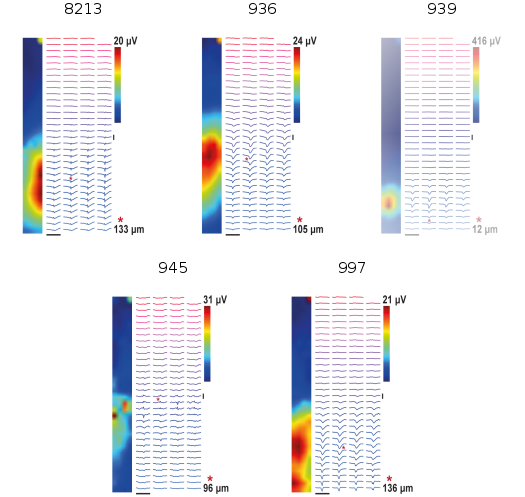
\includegraphics[width=\textwidth]{2.Chapter/dataset-JTA.png}
	\caption{Presentation of the recording used in this project. Here are presented the spatial distribution of the peak-to-peak amplitude of the Juxta-Triggered Averages, illustrated as a interpolated heatmap. In addition, the extracellular JTA waveforms for all the extracellular electrodes are spatially arranged
}
\label{fig:recordings-summary}
\end{figure}


\begin{table}[!h]
\centering
\begin{tabular}{cccccc}
\textbf{Recording ID} & \textbf{Short ID} & \textbf{Distance ($\mu m$) } & \textbf{P2P ($\mu V$)} & \textbf{Depth ($\mu m$)} & \textbf{\# Juxta spikes}\\ \hline
2015\_09\_09\_Pair7.0 & 997 & 136.2 $\pm$ 40 & 20.7 & 1032.8 & 1082  \\ 
2015\_09\_04\_Pair5.0 & 945 & 96.1 $\pm$ 40 & 30.8 & 1185.5 & 185  \\
2015\_09\_03\_Pair6.0 & 936 & 153.3 $\pm$  40 & 24.1 & 1063.2 & 3329 \\
2015\_09\_03\_Pair9.0 & 939 & 11.5 $\pm$  40 & 416.3 & 1152.8 & 5007  \\
2015\_08\_21\_Pair3.0 & 8213 & 132.8 $\pm$ 40 & 19.4 & 1286.0 & 8117 \\ 
\end{tabular}
\caption{Information about the recordings used. The values on the "Recording ID" are conform the dataset provided by \cite{Netoetal}. For convenience, a Short ID will be used throughout this document. P2P stands for Peak-to-Peak Amplitude calculated as the maximum value across electrodes of the difference between the maximum and minimum values of the JTA. In the fifth column are the values of the depth in the cortex. In the last column are the number of spikes detected in the signal from the Juxtacellular pipette.}
\label{tab:sum-recordings}
\end{table}
%$\max_i \left( \max_t \left( JTA_i \right) - \min_t \left( JTA_i \right)\right), i=0,\ldots , 127$
We have some variability in this ensemble. 
The recording 939 was recorded very closed to the neuron and therefore has a very large P2P amplitude and lies above the noise; it also recorded many spikes. 
The recording 945 has a very low count of spikes and relatively low P2P amplitude. For this reason its JTA is not very well defined.
Despite its low P2P amplitude, the recording 8213 is the one with the most events, making its JTA reasonably defined.

In Fig. \ref{fig:recordings-summary}, the spatiotemporal profile of each recording is noticeable and centered around the closest electrode in the probe.
